\documentclass[]{article}
\usepackage{amsmath}
 \usepackage{graphicx}
%opening
\title{Reconciling Information Theory and Probability in Chaotic Dynamics: A Dual-Perspective Analysis of Stochastic Systems}
\author{Ilya Shesterikov}

\begin{document}

\maketitle

\begin{abstract}
This work investigates the fundamental connection between \textbf{information theory/symbolic dynamics} and the statistical description of chaotic dynamical systems, utilizing the fully chaotic Logistic map ($x_{n+1}=4x_{n}(1-x_{n})$) as a foundational model. We explore this relationship through two complementary approaches aimed at reconciling the information-theoretic encoding of trajectories with their probabilistic description. In the first approach, we map the complete set of $2^{12}=4096$ unique symbolic sequences of length $12$ ($12$ cells) back to their corresponding representative initial points in the phase space, demonstrating that the distribution of these representative points exactly reproduces the analytical invariant probability density, $\rho(x)$. In the second approach, we analyze an equidistant ensemble of initial points and observe that the local density of symbolic sequences, quantified by the cluster size $N(x)$, is inversely proportional to $\rho(x)$. Both lines of reasoning unequivocally establish that the density of information encoded by the symbolic sequences is directly proportional to the invariant probability density of the chaotic system.
\end{abstract}

\section{Introduction}

Symbolic dynamics, which involves the encoding of chaotic trajectories using sequences of symbols, constitutes a valuable analytical tool for elucidating the intrinsic nature of chaotic motion. Within this abstract framework, complex patterns and internal relationships inherent in the dynamical system become significantly more tractable and evident.  

In this work, we aim to elucidate the intrinsic connection between information-theoretic principles and the probabilistic description of a stochastic process.
We shall consider two complementary lines of reasoning, aiming to reconcile two perspectives on a stochastic process — one based on information theory and  symbolic dynamics and the other on the probabilistic description.

In the first approach, we analyze all possible ways of encoding chaotic trajectories by unique sequences of symbols. That is, we proceed from the space of symbol sequences toward the corresponding set of chaotic trajectories and their initial conditions.

In the second approach, we move in the opposite direction: starting from a set of chaotic trajectories corresponding to an equidistant ensemble of initial points. This allows us to examine how the symbolic encoding of these trajectories is related to the probabilistic description of the stochastic process.

\section{Chaos and Logistic map}
Specifically, the Logistic map provides an ideal and straightforward paradigm for developing foundational insights into the study of chaotic phenomena.
This map is defined by the following recurrence relation:

\begin{equation}
x_{n+1} = r x_n (1 - x_n)	
\label{fig:logistic_map}
\end{equation}



The map defines a process of iteration, where the output of the function at step $n$ becomes the input for step $n+1$. The sequence of values generated, $\{x_0, x_1, x_2, \dots\}$, is called an \textit{\textbf{orbit}}.
State Variable ($x_n$) - This is the variable whose value evolves over time. Mathematically, it is a real number restricted to the unit interval $I = [0, 1]$. This restriction is necessary to ensure that the next value, $x_{n+1}$, also remains within $[0, 1]$ when the parameter $r$ is in its relevant range $[0, 4]$.
The function $f_r(x)$ is a quadratic polynomial, making the system nonlinear. This nonlinearity is the source of its complex dynamics.
Control parameter ($r$) is a positive real number, typically restricted to $r \in [0, 4]$.
It acts as the "tuning knob" that determines the dynamical properties of the entire system.

To apply symbolic dynamics, the continuous state space (the interval \([0, 1]\)) is divided into a finite number of regions, and each region
 is assigned a \textbf{unique symbol}. An orbit, which is a sequence of real numbers \( x_0, x_1, x_2, \ldots \), is then converted into a \textbf{symbolic sequence} by recording the symbol of the region the trajectory visits at each time step.

A partition is classified as a \textbf{generating partition} if the correspondence between the infinite symbolic sequence and the original orbit is \textbf{one-to-one}. This means that studying the symbolic sequence alone can reveal the essential topological and measure-theoretic properties of the chaotic dynamical system. For one-dimensional maps like the Logistic Map, the boundary points of the partition are determined by the critical points and their preimages under the map.

For the fully chaotic Logistic Map with \( r = 4 \) (i.e., \( x_{n+1} = 4x_n(1 - x_n) \)), the state space \( I = [0,1] \) has a single critical point (the maximum of the parabola) at \( x_c = 0.5 \). The simplest and most fundamental \textbf{generating partition} is the \textbf{binary partition} defined by this critical point:

\begin{itemize}
	\item \textbf{Region 0 (Symbol L or 0)}: \( I_0 = [0, 0.5) \)
	\item \textbf{Region 1 (Symbol R or 1)}: \( I_1 = [0.5, 1] \)
\end{itemize}

The critical point \( x_c = 0.5 \) is the \textit{partition boundary}.

The symbolic sequence \( S = s_0 s_1 s_2 \ldots \) corresponding to an orbit \( x_0, x_1, x_2, \ldots \) is constructed using the following rule:

\[
s_n =
\begin{cases}
	0 \text{ (or L)} & \text{if } x_n \in [0, 0.5) \\
	1 \text{ (or R)} & \text{if } x_n \in [0.5, 1]
\end{cases}
\]

For example, if a trajectory is \( x_0 = 0.2, x_1 = 0.64, x_2 = 0.92, x_3 = 0.29, \ldots \), its symbolic sequence would be \( 0, 1, 1, 0, \ldots \).

Thus, if we take a sequence of 12 iterations, then to each initial point and its trajectory one can associate a certain sequence of symbols. For example, the trajectory of the initial point ($x_0 = 0.2$) can be encoded by the symbolic sequence  $[0,1,1,0,1,0,1,1,1,0,1,0]$. 

\begin{figure}[htbp]
	\centerline{\includegraphics[width=0.5\linewidth]{symbol_sequence.png}}
	\caption{The trajectory of any initial point $x_0$ in the phase space (x) can be mapped to a sequence of symbols consisting of 0s and 1s.}
	\label{fig:symbol_sequence}
\end{figure}

In other words, any initial point in the phase space can be mapped to a sequence of symbols consisting of 0s and 1s, as shown on the figure \ref{fig:symbol_sequence}.
Suppose that each initial point undergoes (N = 12) iterations in the course of its evolution. That is, we have 12 “cells” available to encode all possible trajectories.

\section{First Approach: Mapping From Symbolic Sequences to Chaotic Trajectories}

Let us now consider all possible combinations in the space of these 12 cells.
\begin{equation}
	\begin{gathered}
		[0, 0, 0, 0, 0, 0, 0, 0, 0, 0, 0, 0] \\
		[0, 0, 0, 0, 0, 0, 0, 0, 0, 0, 0, 1] \\
		[0, 0, 0, 0, 0, 0, 0, 0, 0, 0, 1, 0] \\
		[0, 0, 0, 0, 0, 0, 0, 0, 0, 0, 1, 1] \\
		[0, 0, 0, 0, 0, 0, 0, 0, 0, 1, 0, 0] \\
		\vdots \\
		[1, 1, 1, 1, 1, 1, 1, 1, 1, 1, 1, 1]
	\end{gathered}
\label{eq:symbol_sequence}
\end{equation}


 In total, there are ($2^{12}=4096$) such combinations.
Each unique combination corresponds to a unique trajectory and a unique representative initial point. It should be noted, however, that the exact value of the initial point will depend slightly on the chosen reconstruction method, i.e., the procedure is used to map a symbolic sequence back to an initial point. Nonetheless, for any fixed reconstruction method, the resulting set of points will also be unique; there will be no repeated initial points. So, there will be also $4096$ unique initial points.
Let us now ask the question: how are these points distributed in the space of (x)?

The answer is these points will be distributed in space in exactly the same way as the invariant probability density $\rho(x)$ corresponding
to the selected map, in our case the Logistic map. They follow the same law. That is, if one constructs a histogram of the distribution of these initial points, it will reproduce $\rho(x)$, with the only difference that $\rho(x)$ is a normalized quantity. In other words, regions with higher invariant density will contain a higher concentration of representative points, while regions with lower density will contain fewer points. 


\begin{figure}[h!]
	\centering
	\includegraphics[width=\linewidth]{histogramm_symbol_sequence.pdf}
	\caption{Distribution of the representative points of the Logistic map for symbol sequences ranging from $[0, 0, \ldots, 0]$ to $[1, 1, \ldots, 1]$. (a) shows the distribution of the representative points in terms of raw \textbf{Counts}. (b) shows the \textbf{Normalized histogramm}  of the representative points' distribution, which represents the \textbf{Probability density} $P(x)$. The red dashed line in (b) is the \textbf{Analytical density} $\rho(x)$, which closely matches the normalized histogram.}
	\label{fig:histogramm_symbol_sequence}
\end{figure}

This is illustrated in Fig. \ref{fig:histogramm_symbol_sequence}(a). The blue regions show the histogram of initial points generated from the set of symbol sequences
($[0,0,\ldots,0] \rightarrow [1,1,\ldots,1]$)
as defined in (\ref{eq:symbol_sequence}).
Interpreted as a probability distribution, the histogram in Fig. \ref{fig:histogramm_symbol_sequence}(b) is additionally normalized for convenience, so that it satisfies the standard normalization condition. In this way, it visualizes the relative distribution of the representative points across the phase space (x).

\begin{equation}
	\rho(x)=\frac{1}{\pi\sqrt{x(1-x)}}
	\label{eq:invariand_density}
\end{equation}

The red solid curve shows the analytical invariant probability density of the logistic map at control parameter ($r = 4$).
As evident from the figure, the histogram and the analytical density ($\rho(x)$) given in Eq.(\ref{eq:invariand_density}) are in excellent agreement.


The fact that these two distributions coincide is not at all trivial. Let us try to understand why.
Any symbolic sequence can be viewed as an elementary piece of information. Regions where $\rho(x)$ is large correspond to a greater \textbf{\textit{information density}} than regions where it is small. The density of points can therefore be interpreted as the density of information. For this reason, the distribution of representative points mirrors the invariant distribution $\rho(x)$.

\begin{figure}[h!]
	\centering
	\includegraphics[width=0.5\linewidth]{symbol_sequence_linspace.png}
	\caption{Illustration of partitioning the phase space $x \in [0, 1]$ into equally sized intervals. The representative point $x_i$ of an interval is assigned a symbolic sequence. Several distinct nearby points in the phase space, such as the one labeled $x_i$ and its neighbors, may correspond to the same symbolic sequence (e.g., $[0,1,1,0,1,0,0,1,1,0,1,0]$), forming a small cluster of nearby points that are indistinguishable due to the finite symbol resolution.}
	\label{fig:symbol_sequence_linspace}
\end{figure}


\section{Second Approach: From Phase Space (X) to Symbolic Representation}

This question can also be posed differently. 
Consider the uniform discretization of the phase space $x \in [0, 1]$ into a large number of contiguous subintervals, each of equal measure $\Delta x$.
We thus obtain a set of points that are equally spaced. Let each point be assigned a corresponding symbolic sequence $[0, 1, 1, 0, \ldots ]$. It will then turn out that several distinct nearby points may correspond to the same symbolic sequence, as shown in the Figure \ref{fig:symbol_sequence_linspace}. That is, the same sequence will encode not a single point but an \textbf{entire cluster of nearby points} — in fact, a small interval of the phase space. This occurs because, with a finite symbol resolution (e.g., 12 symbols), nearby points cannot be distinguished. The number of symbols determines the resolution.



To each such a cluster, one can assign some representative point $x_i$ lying within that interval (for example, the center of the cluster). 
We will also count how many $\Delta x$ intervals fall into each cluster. Let's designate this quantity as $N$.
 This number characterizes the size of the cluster (in units of $\Delta x$) encoded by the given sequence of symbols.
 Results are shown in the Figure \ref{fig:sequences_within_cluster}.

\begin{figure}[h!]
	\centering
	\includegraphics[width=\linewidth]{sequences_within_cluster.pdf}
	\caption{
Cluster size (N(x)) and the associated uncertainty for a chosen symbolic sequence. The left panel shows how the number of phase-space points mapping to the same symbolic sequence varies across the phase space. Larger values of (N) correspond to larger clusters of indistinguishable points (corresponding to the same symbol sequence). 
The right panel illustrates the inverse quantity (1/N(x)), representing the local informativeness of the symbolic encoding.
 The size of the cluster determines its local informativeness, meaning the longer the encoded interval, the less informative this phase space interval.
The quantity in the figure (a) can be interpreted as a cluster size in units of $\Delta x$ for this particular sequence, which is inversely proportional to the informativeness of this phase space
interval. The inversion of this quantity, namely $1/N$ corresponds to the \textbf{informativeness of the phase space interval}.
It differs from the invariant probability density $\rho(x)$ just by some constant factor, as one can see from the comparison of y log-scale plots shown on the figure (b). 
}
	\label{fig:sequences_within_cluster}
\end{figure}

 The larger this number, the longer the interval encoded by the given sequence of symbols, and thus, the less informative this sequence of symbols will be.
 One can also say that the less informative this particular region of the phase space will be.
 Each symbolic sequence represents one elementary unit (or piece) of information.
 Each symbolic sequence represents one elementary \textbf{unit or piece of information} about the system. 
 The quantity $N(x)$ measures how many nearby points in phase space correspond to that same symbolic sequence, thus quantifying the size of the cluster encoded by a single information unit. 
 Larger $N$ implies lower information content (a less discriminating symbol sequence), while smaller 
 $N$ corresponds to higher resolution in phase space.
  Thus, this quantity is inversely proportional to the \textbf{\textit{local informativeness of the phase space interval}}, i.e., the inversion of this quantity, namely $1/N(x)$ will be our original probability density $\rho(x)$.

This observation is corroborated by the comparison presented in Figure \ref{fig:sequences_within_cluster}(b). In this panel, the quantity 1/N(x) is juxtaposed with the analytical probability density function, $\rho(x)$, defined by Equation \ref{eq:invariand_density}. The use of a logarithmic scale on the y-axis clearly demonstrates that 1/N(x) and $\rho(x)$ exhibit the same functional dependence. The primary distinction between the two quantities is that $\rho(x)$ represents a normalized probability density, whereas 1/N(x) is unnormalized.


\section{Conclusion}

This work successfully reconciled two perspectives—the information-theoretic and the probabilistic—on the intrinsic nature of chaotic motion within the context of the fully chaotic Logistic map. Through the method of symbolic dynamics, we demonstrated a rigorous correspondence between the distribution of information units and the system's statistical properties. Our first key finding, derived from mapping all $2^{12}=4096$ unique symbol sequences to their corresponding initial points, established that the raw count distribution of these representative points mirrors the invariant probability density $\rho(x)$. This shows that regions of higher density are precisely those that contain a greater density of unique symbolic encodings, thus equating probability density with information density in the phase space.The second approach provided a powerful inversion of this concept. By analyzing an equidistant ensemble of initial points, we showed that the size of the cluster, $N(x)$, which represents the set of indistinguishable points mapping to the same symbolic sequence, is inversely proportional to the local informativeness. Crucially, the quantity $1/N(x)$ was shown to exhibit the same functional dependence as the analytical density $\rho(x)$, differing only by a normalization constant.Collectively, these results confirm that for a fully chaotic system with a generating partition, the local informativeness, as measured by the symbolic resolution, is a direct manifestation of the system's inherent probabilistic structure. Future work could extend this dual-perspective analysis to systems requiring higher-order partitions or to non-hyperbolic chaotic systems where the relationship between information density and invariant measure may become more complex.


\end{document}
